\documentclass{tfg_domingo}
% \documentclass[numeros]{tfg_domingo}

\autor{Juan Toca Mateo}
\titulo{Secuencias binarias y sus aplicaciones}
% Título corto para los encabezamientos de pagina:
\corto{Binary sequences and their applications} % En blanco si no es necesario recortarlo.
\ingles{Binary sequences and their applications}
\fecha{septiembre de 2020}
% La normativa prescribe «cuatro o cinco palabras clave, en
% español y en inglés, para su indexación en el repositorio
% de TFG».
\palabras{secuencia, correlacion, señal}%
  {sequence, correlation, signal}

\usepackage{lipsum} % Esto solo es relleno.

\begin{document}

% Si alguna palabra se divide entre dos líneas en un punto
% indebido, podemos indicar aquí los puntos de corte
% aceptables (si los hay), p. ej,
% \hyphenation{ba-rro-co, frío, cria-do, su-per-ra-tón}
\hyphenation{Dijkstra new-speak}

\portada
\frontmatter
% \sucinto{A Sofía}
\gracias{\input{Chapters/agradecimientos.txt}}
\resumen{El análisis de la correlación de señales es una pieza clave en múltiples
desarrollos de ingeniería tales como el GPS, el sónar o la corrección de errores
a la hora de transmitir información. Habiendo moldeado actividades tan diversas
como la conducción, la cartografía o el uso de internet, el estudio de la
función de autocorrelación puede derivar en nuevos desarrollos o mejoras en
los ya existentes. \\

En este proyecto, nos centramos en la generación de nuevas secuencias
pseudoaleatorias mas largas para, entre otros posibles usos, sonares y sistemas
GPS con mayor resolución. Para ello, se ha desarrollado un software desplegable
en un nodo de supercomputación para asistir en la búsqueda de dichas
secuencias.
}{The analisis of the correlation of signals is a key piece in several
engineering developments such as the GPS, the radar or the correction of errors
during information transmission. Having shaped so many diverse activities like
driving, cartography or internet usage, the study of the correlation function
may lead to new developments or improvements in the ones that already exist.\\

In this project, we focus on the generation of new pseudorandom sequences for
more accurate radars or GPS technologies. To do so, a new software, deployable
in a supercomputer, has been developed to assist in the search of these
sequences.
}
\tableofcontents

\mainmatter


\chapter{Introduction}

There is no doubt that signals have changed drastically the way we live.
Physical maps have passed out long ago in favor of real-time position tracking
systems. Who needs a meter when you can send a signal to measure distances
accuratly? Even publishing this project it's thanks to the hard work of
engineers that squeeze the capabilities of the carrier wave to transport
information throughout Internet. \\

In this chapter, we will introduce the correlation, autocorrelation and
crosscorrelation functions for periodic binary sequences and it's mathematical
properties. We will also take a look at pseudorandom noise, it's properties and
practical applications.


\section{Conventions}
 TODO

 %TODO: Add support for correlation with complex numbers

\section{Correlation function}

According to \citet{golomb_ref}, the correlation function measures how similar
two phenomena are. If properly normalized, the function ranges from
+1(identical) to -1(opposite); 0 meaning completly unrelated phenomena.
If we represent those phenomena as vectors, the correlation can be concived
as the normalized dot product between those 2 vectors.
In the discrete case where both sequences have the same length (the one we are
going to focus on), the normalized version is defined as follows:

\begin{definition}[Normalized correlation]\label{def:1}

Given $\alpha$ and $\beta$ two vectors of the same length n and $\alpha_{i}$
and $\beta_{i}$ the components of the vectors:

\begin{equation}\label{eq:1}
C(\alpha , \beta)=\frac{(\alpha \cdot  \beta)}{|\alpha||\beta|}=\frac{\sum_{i=1}^{n} \alpha_{i}\beta_{i}}{(\sum_{i=1}^{n} \alpha_{i}^{2})^{\frac{1}{2}}(\sum_{i=1}^{n} \beta_{i}^{2})^\frac{1}{2}}
\end{equation}
\end{definition}

Notice that in this vector
representation:
\begin{itemize}
  \item Orthogonal vectors have a correlation value of 0
  \item Vectors with the same direction and orientation have a correlation
  value of 1
  \item Vectors with the same direction but opposite orientation have a
  correlation value of -1
\end{itemize}

Even though the normalized version is the best way to represent the degree
of similarity between 2 phenomena and a good way to grasp the concept of
what we are defining, for the rest of the document we are going to use the
unnormalized version if not specified. This version of the correlation function
have several advantages for our research as it is simpler and carries the same
amount of information, saving us some computation resources and complexity on
our theoretical analysis. Keep in mind that it's always posible to move from
applied to the normalized one if we need it. The unnormalized correlation is
defined as:

\begin{definition}[Unnormalized correlation]\label{def:2}
  Given $\alpha$ and $\beta$ two vectors of the same length n and $\alpha_{i}$
  and $\beta_{i}$ the components of the vectors:
  \begin{equation}\label{eq:2}
    C(\alpha , \beta) = (\alpha \cdot  \beta) = \sum_{i=1}^n(\alpha \odot \beta)_{i}= \sum_{i=1}^{n} \alpha_{i}\beta_{i}
  \end{equation}

  Where "$\odot$" represents the pointwise product of vectors.

\end{definition}

Adapting this function from vectors to finite digital signals is straight
forward, as they can be defined in terms of a vector that lives in a vector
space of dimension equal to the length of the signal.


\begin{figure}[ht!] % [h!] fuerza que el elemento se sitúe
                    % en la posición señalada, en vez de al
                    % comienzo de una página.
\begin{center}
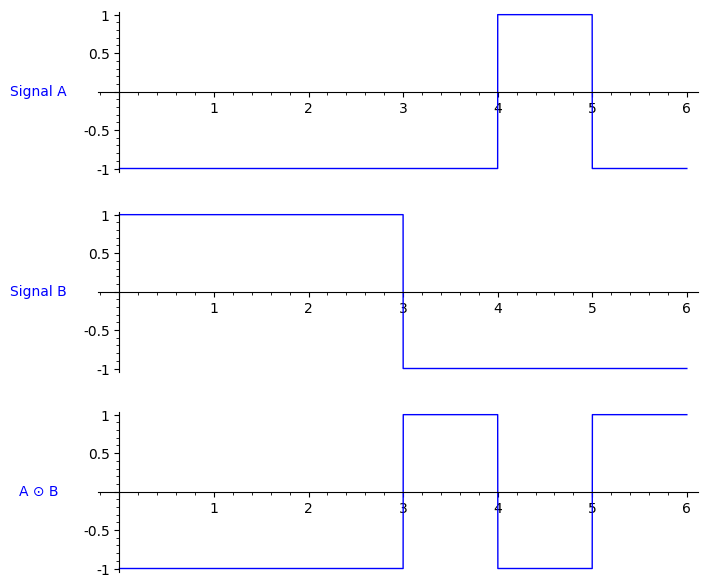
\includegraphics[width=0.7\linewidth]{Chapters/Introduction/signals_correlation}
\end{center}
\caption{Representation of 2 signals an their pointwise product with an unnormalized correlation between them of -2(-1 -1 -1 +1 -1 +1)}
\label{introduction_signals_hadamard}
\end{figure}

If we take a look at Figure \ref{introduction_signals_hadamard}, we can see
a simple computation that can easily be implemented in a chip. Notice that,
in contrast of what would be needed for the normalized version, we only use
integer arithmetics, multiplication and addition rather than squaring along the
signal proccesing and then calculating the square root.











\section{Autocorrelation function}

Going on with the lecture of \citet{golomb_ref}, the autocorrelation function
is a measure of how the correlation behaves if, for a given sequence, a
circular shift is applied and correlated with the original sequence for every
possible shift. It is defined for periodic sequences as follows:

\begin{definition}[Autocorrelation]\label{def:3}

Given the function C defined in Equation \ref{eq:2} and n the length of the
sequence S

\begin{equation}\label{eq:3}
  shift(S, \tau)_i = S_{(i+\tau) \bmod n}
\end{equation}
\begin{equation}\label{eq:4}
  A(S)_{\tau} = C(S, shift(S, \tau)) = \sum_{i=1}^{n}S_{i}S_{(i+\tau) \bmod n}
\end{equation}

\end{definition}

\begin{figure}[ht!] % [h!] fuerza que el elemento se sitúe
                    % en la posición señalada, en vez de al
                    % comienzo de una página.
\begin{center}
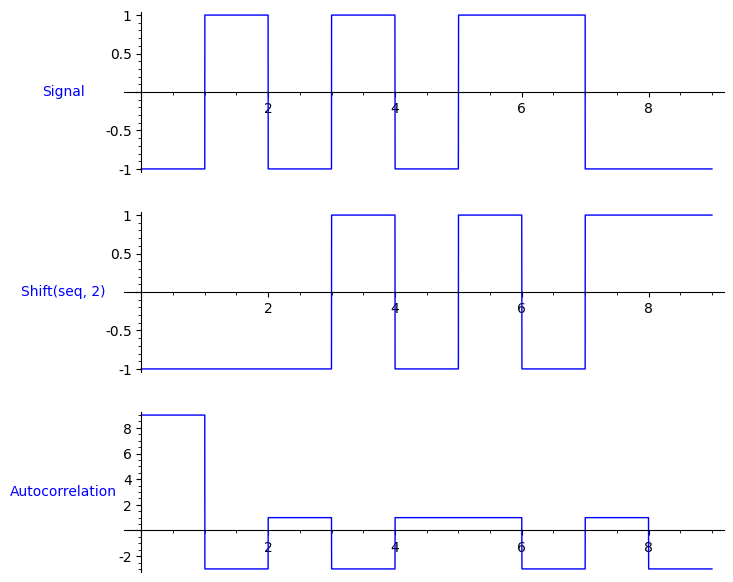
\includegraphics[width=0.7\linewidth]{Chapters/Introduction/signals_autocorrelation}
\end{center}
\caption{A signal with a shifted version of itself and it's autocorrelation function}
\label{introduction_signals_autocorrelation}
\end{figure}

An example of this function is shown in Figure
\ref{introduction_signals_autocorrelation} in which we can find examples of
some important properties of the autocorrelation function:

\begin{theorem}\label{theorem:1.2.1}
  Given a sequence S, the autocorrelation value for $\tau = 1$ is:
    \begin{equation}
      A(S)_{1}=C(S, S)=\sum_{i=1}^{n}S_{i}^2
    \end{equation}
\end{theorem}

\begin{corollary}
  Given the unnormalized autocorrelation of a sequence, we can
  normalize it by dividing it as follows:
  \begin{equation}
    A'(S)_{\tau} = \frac{A(S)_{\tau}}{A(S)_{1}}
  \end{equation}
\end{corollary}

\begin{proof}
  Using Equations \ref{eq:1} and \ref{eq:4}, we can normalize \ref{eq:4} as
  follows:

    $$A'(S)_{\tau} = C'(S, shift(S, \tau)) = \frac{C(S, shift(S, \tau))}{(\sum_{i=1}^{n} S_{i}^{2})^{\frac{1}{2}}(\sum_{i=1}^{n} S_{i+\tau}^{2})^\frac{1}{2}} = \frac{A(S)_{\tau}}{\sum_{i=1}^{n} S_{i}^{2}} = \frac{A(S)_{\tau}}{A(S)_{1}}$$

  Keep in mind that, even though $S_{i}^2$ and $S_{i+\tau}^2$ aren't the same element, the elements of the shifted version are the same as the original sequence so the total sum is the same.
\end{proof}

\begin{corollary}\label{autocorrelation:coro:1}
  Given the autocorrelation of a sequence, $A_{1}(S)$ will always be the maximum value of the autocorrelation.
\end{corollary}

\begin{property}
 Components of the autocorrelation vector belong to the same group as the
  original sequence.
\end{property}

Even though this seems a naive property, this will prove
useful when we introduce the algorithm based in the Fourier Transform to
compute the autocorrelation function.









\section{Crosscorrelation function}

The crosscorrelation function measures how a sequence correlates with all
the posible shifts of another sequence. This function is useful in signal
proccesing to analyze if two signals can be mistaken one for another by a
receiver.


\begin{definition}[Crosscorrelation]\label{def:4}
  Given C the correlation function defined in Equation \ref{eq:2}, shift as the function defined in Equation \ref{eq:3} and n the length of both sequences:
  \begin{equation}\label{eq:7}
    CC(S1, S2)_{\tau} = C(S1, shift(S2, \tau)) = \sum_{i=1}^{n}S1_{i}S2_{(i+\tau) \bmod n}
  \end{equation}
\end{definition}

\begin{figure}[ht!] % [h!] fuerza que el elemento se sitúe
                    % en la posición señalada, en vez de al
                    % comienzo de una página.
\begin{center}
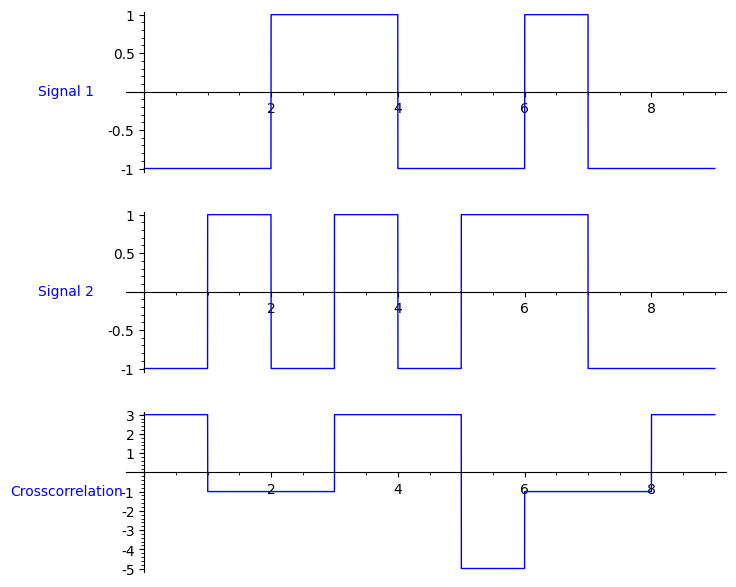
\includegraphics[width=0.7\linewidth]{Chapters/Introduction/signals_crosscorrelation}
\end{center}
\caption{Two signals and it's crosscorrelation}
\label{introduction_signals_crosscorrelation}
\end{figure}

\begin{lemma}\label{lem:1}
  Given a sequence S, CC the crosscorrelation function defined in Equation
  \ref{eq:7} and A the autocorrelation function defined in Equation \ref{eq:4}:
  \begin{equation}\label{eq:8}
    CC(S, S) = A(S)
  \end{equation}
\end{lemma}












\section{Pseudorandom noise(PRN)}

Noise have a different meaning depending on the field of study in which is
used. In our case we are going to work with random vectors of white noise,
which is defined as vectors in which all the components are statistically
independent between them.\cite{white_noise}\\

Even though noise in general is usually seen as an unwanted wave that
limits the amount of information that can be transmited through a
channel\cite{shannon_noise}, it has some practical uses:


\begin{outline}
  \1 PRN-based radars\cite{prn_radar_example1}\cite{prn_radar_example2}
  \1 As the spreading code in direct-sequence spread spectrum(DSSS) \cite{DSSS_1}\cite{DSSS}
    \2 CDMA in wireless communication\cite{DSSS}
    \2 GPS\cite{GPS}
\end{outline}

This practical applications exploit an important noise property:

\begin{property}
  The autocorrelation of a vector of white noise equals 0 for every component
  where $\tau \neq 1$ \cite{everett}
\end{property}

Taking a radar as an example, using this theorem can compute the distance
just by sending a white noise signal to a target and start correlating the
received signal with the original one. As the autocorrelation of
white noise only has a spike when the shift is 0, that spike represents in
which time instant the signal has returned. With that time instant, we can
get the round-trip time and then the actual distance if we know the
propagation speed of the wave.\\

In the case of GPS, the restrictions imposed to the noise sequence are
stronger. First of all, as we will be transmiting several signals in the same
frecuency, we need a set of codes with good crosscorrelation properties
between them. In other words, the crosscorrelation function between two given
codes must trend to 0 in every component, except when $\tau = 1$ and
both codes are the same.\\

As noise is an statistical construct, noise measured from natural phenomena
can generate sequences with poor correlation properties. As both technologies
depend on this properties to work, we must find a way of creating sequences
with properties similar to those of noise in an deterministic and efficient
fashion.\\

This kind of sequences are called Pseudorandom Noise(PRN). In practical
applications, PRN sequences aren't perfect noise because generating it is
difficult and unnecesary. In reality, we don't need an actual 0 in every
position of the autocorrelation. If we let the sequence take values in a
threshold so that the system won't mistake intermidiate values with the
autocorrelation spike, it will behave as expected.

\begin{figure}[ht!] % [h!] fuerza que el elemento se sitúe
                    % en la posición señalada, en vez de al
                    % comienzo de una página.
\begin{center}
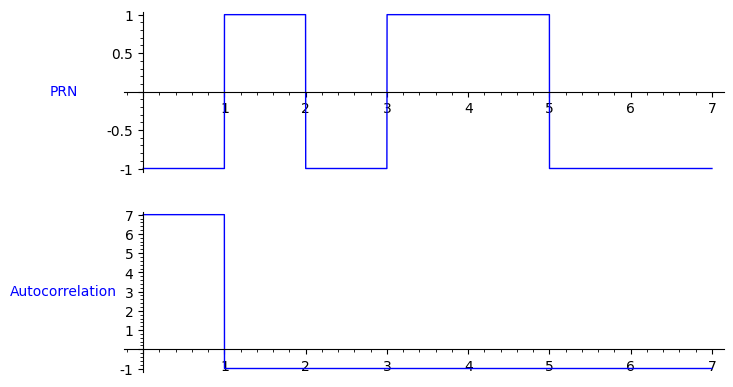
\includegraphics[width=0.7\linewidth]{Chapters/Introduction/signals_prn}
\end{center}
\caption{A pseudorandom noise sequence an it's autocorrelation function.
Notice that this PRN code isn't perfect noise.}
\label{introduction_signals_autocorrelation}
\end{figure}

% TODO Define family of sequences

% TODO Define flat autocorrelation



\chapter{PRN generation}

As explained in the previous chapter, pseudonoise sequences are useful in
tecnologies that need properties similar to those of white noise. In this
chapter, some state-of-the-art tecniques in pseudonoise generation
will be introduced.

\section{Maximum Length Sequence(m-sequences)}

M-sequences are an exponential binary pseudonoise construction that was
initially concived using linear feedback shift registers(LFSR). The particular
type of LFSR used in m-sequences can be simulated with extensions of binary
Finite Fields. The definitions are:

\begin{definition}[LFSR]
  A m-sequence is a binary sequence generated by an LFSR that, given an initial
  state different from 0, it cycles between all posible states except 0.
\end{definition}

Which, as shown in \citet{golomb_ref}, is equivalent to:

\begin{definition}[Finite Fields]
  Given $E/GF(2)$, $\alpha$ a primitive element of $E$ and $S$ the resulting
  sequence:
  \begin{equation}
    S_{i} = trace(\alpha^{i})
  \end{equation}
\end{definition}

\begin{property}
  A m-sequence will always be of length of the form $2^{n}-1$ where n is an
  arbitrary natural number.
\end{property}

\begin{property}
  A m-sequence sequence will always have an autocorrelation function such as
  all the components will be -1 except when $\tau = 1$
\end{property}

\begin{figure}[ht!]
  \inputpython{Chapters/PRN_generation/example_mls.py}{0}{100}
  \caption{An example of a posible implementation of m-sequences}
  \label{mls:fig:1}
\end{figure}

Notice that, even though the construction is exponential, the complexity of
the algorithm is $O(n)$ when $n$ is the size of the sequence. The problem is
that sequences of arbitrary size might be needed in some applications. As it will
be discussed see in a following chapter, the complexity of computing the
autocorrelation with the Fourier Transform approach is $O(n*log(n))$ so using longer
sequences than needed has a direct impact on the performance of the system. \\

This sequences by themselves might not a be huge deal because they don't define
a way to build families of well crosscorrelated sequences, but they are the
building blocks for other contructions, such as the Gold Codes used in GPS and
CDMA.

\section{Gold Codes}

Gold codes\cite{gold_codes} are a family of sequences, derived from
m-sequences, with very important properties that are used in several
applications such as wireless communication and geolocalisation. A Gold Code
generator gets two m-sequences sequences that fulfill:

\begin{property}
  Given two m-sequences that can generate Gold Codes, $S1$ and $S2$, of length
  $2^{n}-1$, $CC$ the crosscorrelation function defined in Equation \ref{eq:7}:
    \begin{equation}\label{gold:eq:1}
      max |CC(S1, S2)| \leq 2^{\frac{n+2}{2}}
    \end{equation}
\end{property}

And XORs all their relative shifts generating a family of $2^{n} + 1$ sequences
($2^{n} - 1$ XORed sequences + 2 m-sequences).

\begin{property}
  Given any two sequences, S1 and S2, from a Gold family of sequences of length
  $2^{n}-1$, $CC$ the crosscorrelation function defined in Equation \ref{eq:7}:
  \begin{equation}
        max |CC(S1, S2)| \leq \left\{\begin{array}{lr}
            2^{\frac{n+2}{2}}+1 & \textnormal{ if n is even } \\
            2^{\frac{n+1}{2}}+1 & \textnormal{ if n is odd } \\
        \end{array}\right.
  \end{equation}
\end{property}

% TODO: Add a  code example

This property means that the crosscorrelation between any given pair of
sequences from a Gold family is low enough to differentiate them. This proves
useful when several devices are transmiting in the same frecuency and we must
treat signals that are not the one we want to receive as noise.\\

Gold also showed  a way to generate this pair of sequences,
using a decimation of one m-sequence.

\begin{definition}[Decimation]
  Given a sequence $S$ of length $n$, a decimation by $q$ of $S$ is defined as:
  \begin{equation}
    S[q]_{i} = S_{((q·i) \bmod n)}
  \end{equation}
\end{definition}

\begin{property}
  Given a m-sequence $S$ of length $2^n - 1$ where n is odd and and a
  coprime of $n$ named $k$, the sequence pair $(S, S[2^{k} + 1])$ number
  fulfills equation \ref{gold:eq:1}.
\end{property}

\begin{figure}[ht!]
  \inputpython{Chapters/PRN_generation/example_gold.py}{0}{100}
  \caption{An example implementation of a generation of a family of gold
  sequences relying in the example at Figure \ref{mls:fig:1}.}
  \label{}
\end{figure}

Notice that this construction has the same problem as m-sequences. It's
an exponential contruction so it might not be enough for some applications.

\section{Legendre sequences}

Legendre sequences, as explained in \citet{legendre_sequences}, are binary
sequences defined through quadratic residues as follows:

\begin{definition}
  Let $p$ be an odd prime and the function "Legendre Symbol" be:
    \begin{equation}
      LSy(n, p) = \left\{\begin{array}{lr}
          1  & \textnormal{if n is a quadratic residue mod p}   \\
          -1 & \textnormal{otherwise} \\
      \end{array}\right.
    \end{equation}
  We define the Legendre Sequence as:
    \begin{equation}
      LSs(p)_{i} = LSy(i-1, p) \textnormal{  where  } 1 < i \leq p
    \end{equation}
\end{definition}

\begin{figure}[ht!]
  \inputpython{Chapters/PRN_generation/example_legendre.py}{0}{100}
  \caption{An example implementation of the generation of a Legendre sequence.}
  \label{}
\end{figure}

Some Legendre Sequences have interesting autocorrelation properties:
\begin{property}\label{property:2.3.1}
  Given an odd prime $p$ such as $p \equiv 3 \bmod 4$, we can say that
  $LSs(p)$ has a flat autocorrelation.\cite{legendre_sequences}
\end{property}

Even though \citet{legendre_sequences} has a generalization of property
\ref{property:2.3.1} to all Legendre Sequences, it requires the introduction of
a third symbol making the sequence non-binary. \\

As $p$ is the variable defining the size of the generated sequence, we can
derive that the distribution of Legendre Sequences is related to the Prime
Number Theorem. This means that Legendre Sequences have more possible lengths
than in m-sequences or other exponential contructions. However, Legendre
Sequences have the drawback that there is only one per sequence length.

\section{Composition method}

\subsection{Algorythm}

The composition method uses a base sequence and a sequence of shifts to
create a matrix of sequence components as follows:

\begin{definition}[Composite matrix]
  Given a base sequence $S$ of length $n$ and a sequence of integers $T$ of
  length $m$ such that:
  \begin{equation}\label{composition:eq:1}
    0 \leq T_{i} < n
  \end{equation}
  \begin{equation}\label{composition:eq:2}
    gcd(n, m) = 1
  \end{equation}

  Given the $shift$ function defined in Equation \ref{eq:3},
  we define the composite matrix as:

  \begin{equation}\label{composition:eq:3}
    CM(S, T) = \begin{bmatrix}
      shift(S, T_{0})_{0} & shift(S, T_{1})_{0} & \dots & shift(S, T_{m-1})_{0} \\
      shift(S, T_{0})_{1} & shift(S, T_{1})_{1} \\
      \vdots & & \ddots \\
      shift(S, T_{0})_{n-1} & & & shift(S, T_{m-1})_{n-1}
    \end{bmatrix}
  \end{equation}

  In other words, each column represents a shift of the base sequence defined
  by the sequence of shifts.
\end{definition}

\begin{definition}[Composite sequence]
  Given a base sequence $S$ of length $n$ and a sequence of integers $T$ of
  length $m$ that fulfill Equations \ref{composition:eq:1} and
  \ref{composition:eq:2} and the composite matrix defined at Equation
  \ref{composition:eq:3}, we define the composite sequence as:
  \begin{equation}
    CS(S, T)_{i} = CM(S, T)_{(i \bmod m), (i \bmod n)}
  \end{equation}
\end{definition}

\begin{figure}[ht!]
  $$S = \begin{bmatrix}
    0 & 1 & 2 & 3 & 4\\
  \end{bmatrix}$$
  $$T = \begin{bmatrix}
    0 & 2 & 1 & 4 & 3 \\
  \end{bmatrix}
  $$
  $$CM(S, T) = \begin{bmatrix}
  0 & 3 & 4 & 1 & 2 & 4\\
  1 & 4 & 0 & 2 & 3 & 0\\
  2 & 0 & 1 & 3 & 4 & 1\\
  3 & 1 & 2 & 4 & 0 & 2\\
  4 & 2 & 3 & 0 & 1 & 3\\
  \end{bmatrix}
  $$
  $$CS(S, T) = \text{[0 4 1 4 1 4 1 0 2 0 2 0 2 1 3 1 3 1 3 2 4 2 4 2 4 3 0 3 0 3]}\\
  $$
  \caption{Example of a computation of the composition method(note that we are
  using a non-binary sequence to illustrate better the method)}
  \label{}
\end{figure}

\subsection{Costas arrays}

Costas arrays, discovered independently by John P. Costas\cite{costas_costas}
and E.N. Gilbert \cite{gilbert_costas} in 1965, are a set of sequences highly
used in radar and sonar applications. We are going to provide the 2 definitions
as both will be useful for different purposes:

\begin{definition}[Costas array(Costas)]
  Square matrix of size $n×n$ filled with 0s and 1s such that there
  aren't more than multiple 1s in each row or column and that every
  displacement vector is distinct from the rest.
\end{definition}

This definition is used in several deployments of sonar and radar to generate
systems with a good ambiguity function, in other words, tolerant to Doppler
effect.

\begin{figure}[ht!]
  $$
  \begin{bmatrix}
   1&0&0&0\\
   0&0&0&1\\
   0&1&0&0\\
   0&0&1&0
  \end{bmatrix}
  $$
  \caption{An example of a Costas array}
  \label{fig:costas_1}
\end{figure}

Notice that we could compact the representation by just having a list of the
rows in which each 1 lives:

\begin{figure}[ht!]
  $$[4, 2, 1, 3]$$
  \caption{The compact representation of the Costas array of Figure
  \ref{fig:costas_1}}
  \label{fig:costas_2}
\end{figure}

This representation is equivalent to the definition of a Costas array provided
by Gilbert:

\begin{definition}[Distinct difference permutations]\label{def:costas_1}
  Given a sequence of integers $S$ of length $n$ such that:
    \begin{equation}\label{eq:costas_1}
      0 \leq S_{i} < n
    \end{equation}
  We say that $S$ is a distinct difference permutation $r$ apart if,
  for any given pair $(S_{i}, S_{j})$, satisfies:
    \begin{equation}\label{eq:costas_2}
      S_{i} - S_{i+r} \not \equiv S_{j} - S_{j+r} \bmod n
    \end{equation}
\end{definition}

\begin{definition}[Costas array(Gilbert)]
  Given a sequence $S$ satisfying Equation \ref{eq:costas_1}, we say it's a
  Costas array if, for any given $r$ value, it satisfies Equation
  \ref{eq:costas_2}.
\end{definition}

This compact representation can be feeded into the composition method as
a sequence of shifts generating interesting new sequences. [citation needed]\\

Several construction methods have
been proposed. For sake of simplicity, we are going to introduce just the Welsh
construction as defined in Gilbert \cite{gilbert_costas}:\\

Given a prime number $p$ and a primitive root $g$ of $p$, we can contruct a
Costas array $S$ as follows:
\begin{equation}
  S_{i} \equiv g^{i} \bmod p
\end{equation}

Notice that this contruction can generate sequences of a prime length as in
the Legendre Sequences. However, it can generate several sequences for a given
length. As the number of possible sequences depend on the number of primitive
elements of the finite field of order $p$, the number of possible costas arrays
for a given length using this construction is $\phi(p-1)$ where $\phi$ is the
Euler's totient function.



\backmatter
% Indique aquí el fichero .bib que contenga su bibliografía.
\bibliography{refs}

\end{document}
